\documentclass[a4paper, 11pt]{article}
\author{Kajetan Kaczmarek}
\usepackage{amsmath}
\usepackage[T1]{fontenc}
\usepackage[utf8]{inputenc}
\usepackage{graphicx}
\usepackage[polish]{babel}
\graphicspath{ {C:/Users/Kajkacz/Desktop/Projekty/MNUM/Numerical-Methodes/Images/} }

\begin{document}
\title{Sprawozdanie MNUM \\* Projekt nr.1 \\* 
Zadanie 1.1 \\*}
\maketitle

\begin{enumerate}

\item Opis zastosowanych algorytmów : 
\begin{enumerate}
\item Do sprawdzenia dokładności maszynowej komputera wykorzystałem prosty algorytm dzielący liczbę 1 przez 2 przy każdej kolejnej iteracji tak długo aż nie była ona równa 0.Dla mojego komputera otrzymałem wynik 1076
\item Przy drugim poleceniu wykorzystałem algorytm faktoryzacji Cholesky'ego Banachiewicza. Najpierw utworzyłem funkcje generateA, generateB oraz generateC, tworzące zbiory danych zgodnie z podanymi specyfikacjami.Następnie użyłem pomocniczych funkcji do faktoryzacji
 Cholesky'ego zgodnie z podanymi wzorami 
 \[ l_{ii} = \sqrt{a_{ii} - \sum_{ k = 1 }^{i-1}l^2_{ik} }  \]
  oraz 
 \[ l_{ji} =
  \dfrac
 { a_{ji} - \sum_{k=1}^{i-1}
  l_{jk} \cdot l_{ik}}{l_{ii} } \]
  Otrzymałem dzięki temu macierz która pomnożona przez swoją tranzpozycję odtworzy zadaną macierz A.Następnie używam otrzymanej macierzy L do rozwiązania równania. Błędy dla kolejnych, coraz większych, iteracji, kształtują się następująco :

\item W metodzie Gaussa-Siedel'a rozbijamy zadaną macierz na trzy - L - część pod przekątną , D - wyłącznie przekątną oraz U - część ponad przekątną. W moim programie służy do tego podfunkcja decompose.Następnie przeprowadzamy kolejne iteracje modelu \[ Dx*{(i+1)} = -Lx*{(i+1)} - Ux*{(i)} + b \] 
Dzięki faktowi że połowa macierzy L jest wypełniona zerami, zachowując odpowiedni porządek, możemy użyć ww. wzoru pomimo występowania po prawej stronie elementów x+1
\end{enumerate}
\item Wydruki programów
\begin{center}

\begin{enumerate}
	\item Program 1 - Sprawdzenie dokładności maszynowej \\*
	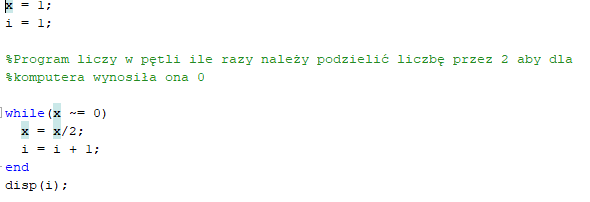
\includegraphics[width=1\linewidth]{P1}
	\item Program 2 - Rozwiązanie układu równań metodą faktoryzacji Cholesky'ego-Banachiewicza
	\begin{itemize}
	\item Główna funkcja (wrapper) dla drugiego zadania  \\* 	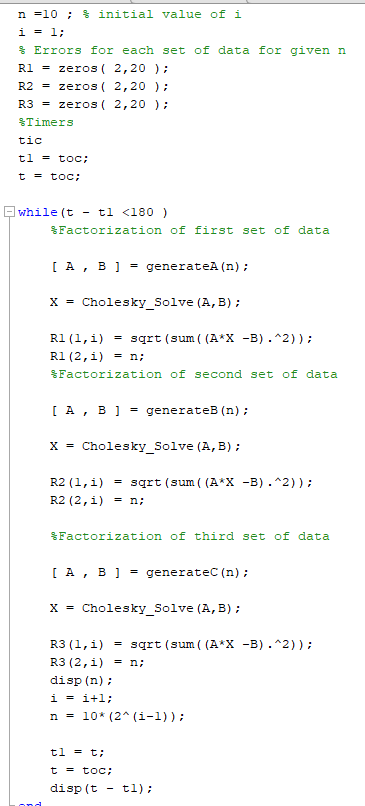
\includegraphics[width=1\linewidth]{P2_main}	
	\item 	Generator zbioeru danych A \\*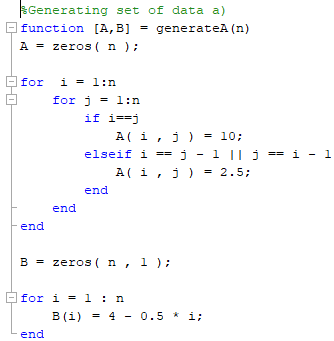
\includegraphics[width=1\linewidth]{P2_generateA}
	\item 	Generator zbioeru danych B \\*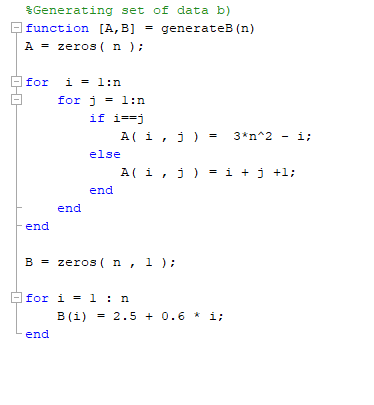
\includegraphics[width=1\linewidth]{P2_generateB}
	\item 	Generator zbioeru danych C \\*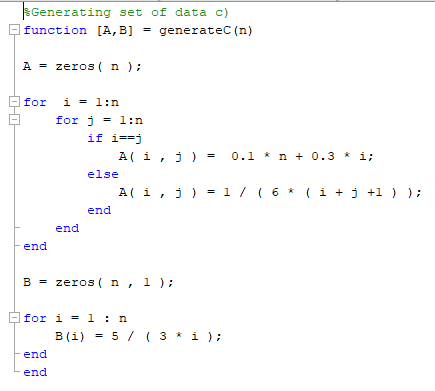
\includegraphics[width=1\linewidth]{P2_generateC}
	\item 	Funkcja faktoryzująca \\* 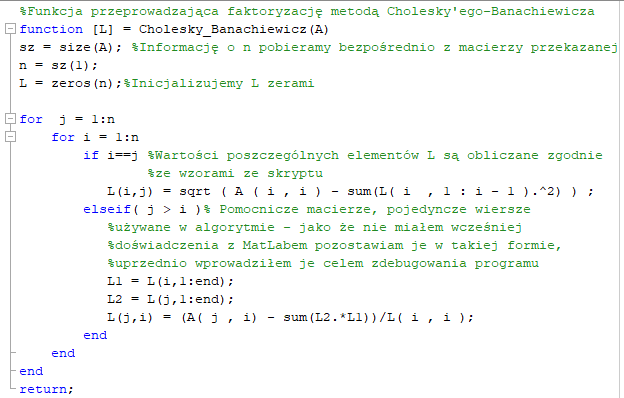
\includegraphics[width=1.5\linewidth]{P2_Faktoryzacja}
	\item 	 Propagacja wsteczna\\*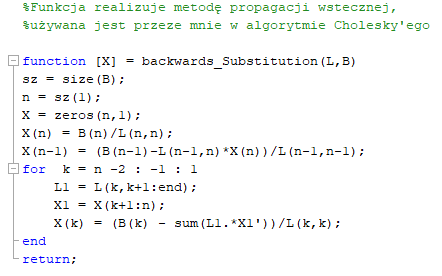
\includegraphics[width=1.5\linewidth]{P2_back}
	\item 	Propagacja wprzód  \\*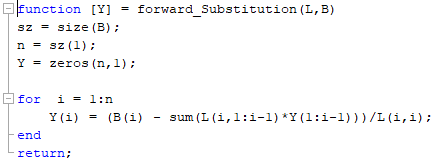
\includegraphics[width=1\linewidth]{P2_fore}
	\item  Funckja rozwiązująca równania  \\*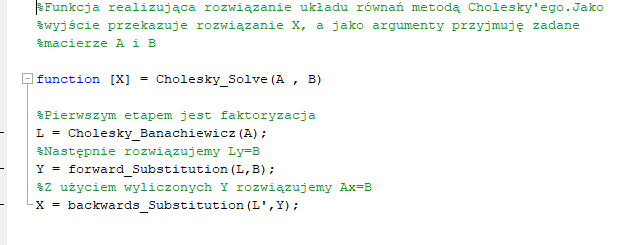
\includegraphics[width=1\linewidth]{P2_solve}
\end{itemize}	
	\item Program 3 - Rozwiązanie układu równań metodą Gaussa-Seidela
	\begin{itemize}
	\item Główna funkcja (wrapper) dla trzeciego zadania  \\* 	
	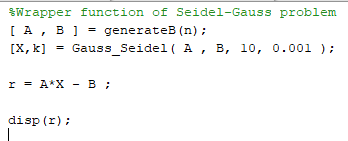
\includegraphics[width=1\linewidth]{P3_main}
	\item Funkcja rozkładająca na 3 macierze\\* 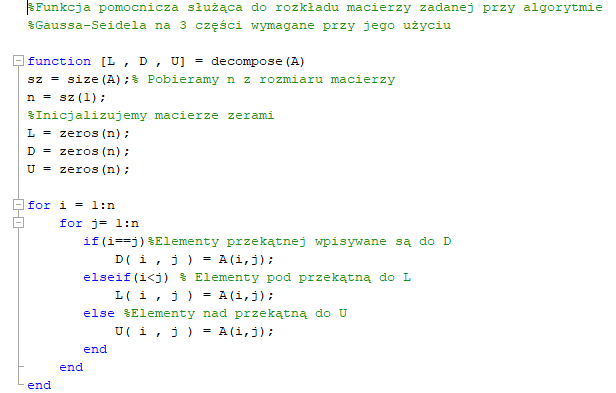
\includegraphics[width=1\linewidth]{P3_decompose}
	\item Funkcja rozwiązująca równania \\*	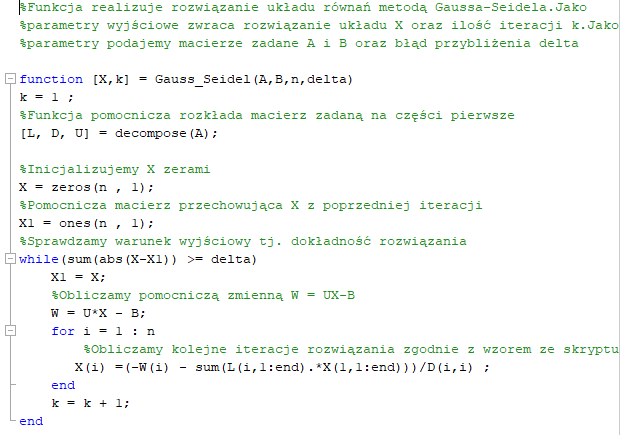
\includegraphics[width=1\linewidth]{P3_solve}
	\end{itemize}
	\end{enumerate}
\end{center}




\item Wyniki oraz wnioski
\begin{itemize}
\item Dla pierwszego algorytmu otrzymałem wynik rzędu ponad 1000 (dokładnie 1076) Liczba ta wydaje mi się bardzo duża. niemniej algorytm jest prosty i nie mogę doszukać się w nim błędu
\item Jeśli chodzi o drugie zadanie, zadany czas 3 minut został przekroczony dla n>2560. Otrzymałem następujące wyniki normy residuum -
\begin{itemize}
\item Zbiór danych 1 \\* 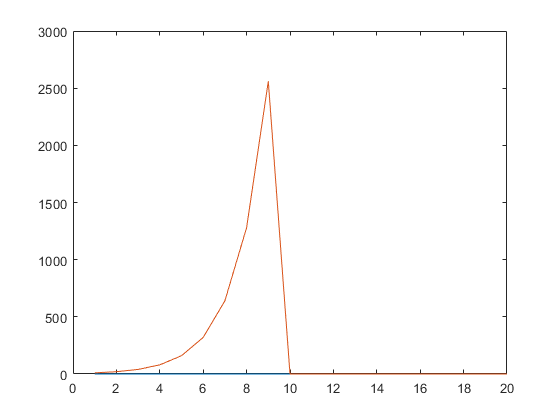
\includegraphics[width=1\linewidth]{Plot1}
\item Zbiór danych 2 \\* 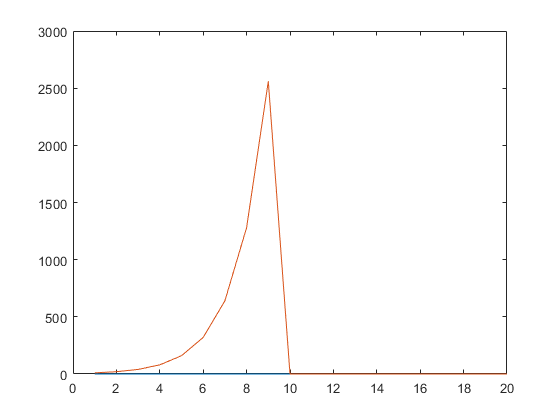
\includegraphics[width=1\linewidth]{Plot2}
\item Zbiór danych 3 \\* 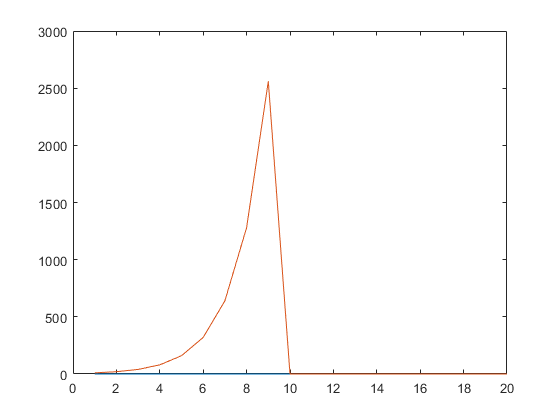
\includegraphics[width=1\linewidth]{Plot3}
\end{itemize}
\item Jak widać, dane są bardzo zbliżone dla wszystkich zestawów danych - rokuje to na korzyść algorytmu.Z drugiej strony, błąd wzrastał stale aż do zakończenia pracy algorytmu - prawa strona, równa 0, to elementy dla których nie znaleziono rozwiązania z powodu przekroczenia czasu
\item Dla trzeciego zadania otzymałem błędy rzędu około ~15
\end{itemize}
\end{enumerate}
\end{document}
